\documentclass[journal,12pt,twocolumn]{IEEEtran}

\usepackage{setspace}
%\usepackage{gensymb}
\singlespacing
\usepackage[cmex10]{amsmath}

\usepackage{amsthm}
\usepackage{tikz}
\usepackage{mathrsfs}
\usepackage{txfonts}
%\usepackage{stfloats}
\usepackage{bm}
\usepackage{cite}
%\usepackage{cases}
\usepackage{subfig}

\usepackage{longtable}
%\usepackage{multirow}

%\usepackage{enumitem}
\usepackage{mathtools}
%\usepackage{steinmetz}
%\usepackage{tikz}
\usepackage{tikz}
\usepackage{circuitikz}
\usepackage{verbatim}
%\usepackage{tfrupee}
\usepackage[breaklinks=true]{hyperref}
\usepackage{graphicx}
%\usepackage{tkz-euclide}

\usetikzlibrary{calc,math}
\usepackage{listings}
    \usepackage{color}                                            %%
    \usepackage{array}                                            %%
    \usepackage{longtable}                                        %%
    \usepackage{calc}                                             %%
    %\usepackage{multirow}                                         %%
    \usepackage{hhline}                                           %%
    \usepackage{ifthen}                                           %%
    \usepackage{lscape}     
\usepackage{multicol}
%\usepackage{chngcntr}

\DeclareMathOperator*{\Res}{Res}

\renewcommand\thesection{\arabic{section}}
\renewcommand\thesubsection{\thesection.\arabic{subsection}}
\renewcommand\thesubsubsection{\thesubsection.\arabic{subsubsection}}

\renewcommand\thesectiondis{\arabic{section}}
\renewcommand\thesubsectiondis{\thesectiondis.\arabic{subsection}}
\renewcommand\thesubsubsectiondis{\thesubsectiondis.\arabic{subsubsection}}


\hyphenation{op-tical net-works semi-conduc-tor}
\def\inputGnumericTable{}                                 %%

\lstset{
%language=C,
frame=single, 
breaklines=true,
columns=fullflexible
}
\begin{document}


\newtheorem{theorem}{Theorem}[section]
\newtheorem{problem}{Problem}
\newtheorem{proposition}{Proposition}[section]
\newtheorem{lemma}{Lemma}[section]
\newtheorem{corollary}[theorem]{Corollary}
\newtheorem{example}{Example}[section]
\newtheorem{definition}[problem]{Definition}

\newcommand{\BEQA}{\begin{eqnarray}}
\newcommand{\EEQA}{\end{eqnarray}}
\newcommand{\define}{\stackrel{\triangle}{=}}
\bibliographystyle{IEEEtran}
\raggedbottom
\setlength{\parindent}{0pt}
\providecommand{\mbf}{\mathbf}
\providecommand{\pr}[1]{\ensuremath{\Pr\left(#1\right)}}
\providecommand{\qfunc}[1]{\ensuremath{Q\left(#1\right)}}
\providecommand{\sbrak}[1]{\ensuremath{{}\left[#1\right]}}
\providecommand{\lsbrak}[1]{\ensuremath{{}\left[#1\right.}}
\providecommand{\rsbrak}[1]{\ensuremath{{}\left.#1\right]}}
\providecommand{\brak}[1]{\ensuremath{\left(#1\right)}}
\providecommand{\lbrak}[1]{\ensuremath{\left(#1\right.}}
\providecommand{\rbrak}[1]{\ensuremath{\left.#1\right)}}
\providecommand{\cbrak}[1]{\ensuremath{\left\{#1\right\}}}
\providecommand{\lcbrak}[1]{\ensuremath{\left\{#1\right.}}
\providecommand{\rcbrak}[1]{\ensuremath{\left.#1\right\}}}
\theoremstyle{remark}
\newtheorem{rem}{Remark}
\newcommand{\sgn}{\mathop{\mathrm{sgn}}}
\providecommand{\abs}[1]{\left\vert#1\right\vert}
\providecommand{\res}[1]{\Res\displaylimits_{#1}} 
\providecommand{\norm}[1]{\left\lVert#1\right\rVert}
%\providecommand{\norm}[1]{\lVert#1\rVert}
\providecommand{\mtx}[1]{\mathbf{#1}}
\providecommand{\mean}[1]{E\left[ #1 \right]}
\providecommand{\fourier}{\overset{\mathcal{F}}{ \rightleftharpoons}}
%\providecommand{\hilbert}{\overset{\mathcal{H}}{ \rightleftharpoons}}
\providecommand{\system}{\overset{\mathcal{H}}{ \longleftrightarrow}}
	%\newcommand{\solution}[2]{\textbf{Solution:}{#1}}
\newcommand{\solution}{\noindent \textbf{Solution: }}
\newcommand{\cosec}{\,\text{cosec}\,}
\providecommand{\dec}[2]{\ensuremath{\overset{#1}{\underset{#2}{\gtrless}}}}
\newcommand{\myvec}[1]{\ensuremath{\begin{pmatrix}#1\end{pmatrix}}}
\newcommand{\mydet}[1]{\ensuremath{\begin{vmatrix}#1\end{vmatrix}}}
\numberwithin{equation}{subsection}
\makeatletter
\@addtoreset{figure}{problem}
\makeatother
\let\StandardTheFigure\thefigure
\let\vec\mathbf
\renewcommand{\thefigure}{\theproblem}
\def\putbox#1#2#3{\makebox[0in][l]{\makebox[#1][l]{}\raisebox{\baselineskip}[0in][0in]{\raisebox{#2}[0in][0in]{#3}}}}
     \def\rightbox#1{\makebox[0in][r]{#1}}
     \def\centbox#1{\makebox[0in]{#1}}
     \def\topbox#1{\raisebox{-\baselineskip}[0in][0in]{#1}}
     \def\midbox#1{\raisebox{-0.5\baselineskip}[0in][0in]{#1}}
\vspace{3cm}

\title{Assignment-1 (EE4013)}
\author{EE18BTECH11013 - Divyansh Maduriya}
\maketitle
\newpage
\bigskip
\renewcommand{\thefigure}{\theenumi}
\renewcommand{\thetable}{\theenumi}
Download c codes from 
\begin{lstlisting}
https://github.com/Divyansh-28/EE18BTECH11013-EE-4013/tree/master/code
\end{lstlisting}
%
and latex-tikz codes from 
%
\begin{lstlisting}
https://github.com/Divyansh-28/EE18BTECH11013-EE-4013/tree/master
\end{lstlisting}
\section{Problem}


	consider a complete binary tree with 7 nodes. Let A denote the set of first 3 elements obtained by performing Breadth-First search (BFS) starting from root. Let B denote the set of first 3 elements obtained by performing Depth first Search(DFS) starting from the root. 
	the value of$$|A-B|$$ is ?
	
\section{Solution}

Let us start with drawing a 7 node binary tree, then we'll run BFS and DFS from the root node respectively to get set A and B.


\begin{figure}[!h]
\centering
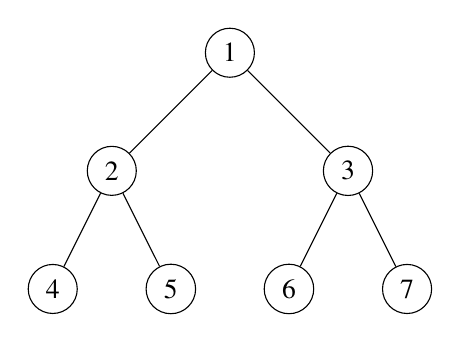
\begin{tikzpicture}[level/.style={sibling distance=30mm/#1}]
\node [circle,draw] (z){1}
  child {node [circle,draw] (a) {2}
    child {node [circle,draw] (b) {4}}
    child {node [circle,draw] (g) {5}}
  }
  child {node [circle,draw] (j) {3}
    child {node [circle,draw] (k) {6}}
  child {node [circle,draw] (l) {7}}
};
\end{tikzpicture}
\caption{Binary Tree} \label{fig:M1}
\end{figure}

Representing the nodes of the binary tree above in the form of an array in the following way.

\begin{align}
   Arr B = [1,2,3,4,5,6,7]
\end{align}\\
Now, Let's traverse through the array
covering the BFS nodes/indexes starting from the root node.

\begin{align}
i =i+1
\end{align}\\

Where, i represents a particular node/index, starting from i=0(i.e root node).

\vspace{1cm}

 Now, Let A denote the set of first 3 elements of BFS.
Therefore,
\begin{align}
A = \{1,2,3\} 
\end{align}
Similarly, Let's traverse through the array
covering the DFS nodes/indexes starting from the root node.
\begin{align}
i =2i+1
\end{align}\\

Where, i represents a particular node/index, starting from i=0(i.e root node)

\vspace{1cm}

Now, Let B denote the set of first 3 elements of DFS.
Therefore,

\begin{align}
  B = \{1,2,4\}   
\end{align}\\
Now,
\begin{align}
    A-B = \{3\}
\end{align}\\
and \\
\begin{align}
    $$|A-B|$$ = 1
\end{align}\\

C Code snippets of the BFS and DFS functions :
\vspace{0.5cm}

BFS C function:

\begin{align}

\begin{lstlisting}

    int *bfs(int * tree) { 
    int * set = (int* ) malloc(1*sizeof(int)); 
    int  i = 0;
    setbfssz = 0; 
    while(setbfssz<3) { 
    
      set = (int *)realloc(set, (setbfssz+1)*sizeof(int)); 
      set[setbfssz]  = tree[i]; 
      i++; 
      setbfssz++; 
    } 
    return set; 
}
\end{lstlisting}
 
\end{align}

DFS C function:

\begin{align}
 
 \begin{lstlisting}
 int * dfs(int * tree) { 
    int * set = (int* ) malloc(1*sizeof(int));
    int  i = 0; 
    setdfssz = 0; 
    while(setdfssz < 3) { 
    
      set = (int *)realloc(set, (setdfssz+1)*sizeof(int));  
      set[setdfssz]  = tree[i];  
      i = 2*i+1; 
      setdfssz++;  
    } 
    return set;  
}
 
\end{lstlisting}
    
\end{align}


\end{document}